\documentclass[a4paper,12pt]{article}
\usepackage[utf8]{inputenc}
\usepackage[francais]{babel}
\usepackage[T1]{fontenc}
\usepackage[pdftex]{graphicx}
\usepackage{url}


\setlength{\parindent}{0cm}
\setlength{\parskip}{1ex plus 0.5ex minus 0.2ex}
\newcommand{\hsp}{\hspace{20pt}}
\newcommand{\HRule}{\rule{\linewidth}{0.5mm}}
%opening


\begin{document}

\begin{titlepage}
  \begin{sffamily}
  \begin{center}

    % Upper part of the page. The '~' is needed because \\
    % only works if a paragraph has started.
    
\includegraphics[scale=1]{univangers.jpg}~\\[1.5cm]

    \textsc{\LARGE Université d'Angers}\\[2cm]

   

    % Title
    \HRule \\[0.4cm]
    { \huge \bfseries Installations de logiciels :}{ \bfseries  \\ dépendance, dépôt, gestionnaire de package, installation depuis les sources, environnement virtuel python\\[0.4cm] }

    \HRule \\[2cm]
    \\[2cm]
    

    % Author and supervisor
    \begin{minipage}{0.4\textwidth}
      \begin{flushleft} \large
        CHERRUAU \textsc{Anthony}\\
        POUPELIN \textsc{Bastien}\\
        THEBAUDIN \textsc{Corentin}\\
      \end{flushleft}
    \end{minipage}
    

    \vfill
\HRule\\[2cm]
    % Bottom of the page
    {\large 16 novembre 2016}

  \end{center}
  \end{sffamily}
\end{titlepage}
\clearpage

\tableofcontents

\clearpage



\section{Dépendance}
\paragraph{}
Les programmes informatiques ne sont pas des briques logicielles isolées : ils s’utilisent les uns les autres, de façon
à réduire tant les ressources utilisées par l’ensemble du processus aboutissant à leur exécution (installation sur disque, mise en mémoire, ...), 
que le temps de codage nécessaire aux programmeurs pour les réaliser. Par exemple, lorsqu’un logiciel lit ou écrit sur un disque, 
il utilise un sous-programme système existant dans une librairie.\\

Par extension un certain nombre de programmes utilitaires, automatisant de nombreuses fonctions récurrentes, 
sont disponibles dans des fichiers librairies partagés (appelés en l’occurrence, Shared Library).\\

Les programmes peuvent intégrer les sous programmes contenus dans les librairies de deux façons, soit de manière statique ou de manière dynamique.\\

De manière statique toutes les sous programmes des librairies sont inclus dans le programme lors de son chargement en mémoire centrale 
(la taille mémoire centrale nécessaire au programme est donc plus grande).\\

De manière dynamique, lors de l’usage d’un sous programme, le programme le charge en mémoire à partir de la librairie qui le contient.\\

Différents programmes, de différents logiciels, sont donc susceptibles d’utiliser à tout moment des librairies identiques. 
Celles-ci sont donc identifiées avec précision  et stockées sur disque suivant une arborescence déterminée.\\

Certaines des distributions GNU/Linux, utilisant les systèmes « rpm » (Redhat, Mandrake) ou « deb » (Debian), gèrent 
les « dépendances » entre les logiciels utilisateurs et les librairies de sous programmes disponibles. 
Ce système de gestion des dépendances n’est donc pas inhérent à Linux (noyau dirait-on) mais lié à l’usage de certaines distributions. 
Malgré tout, sur des distributions ne gérant pas les dépendances, comme la Slackware, l’installation de packages de type tarball (extension .tgz)
permet, grâce à des programmes spécifiques (installpkg, pkgtools, removepkg, ...) , de garder une trace de l’installation des logiciels installés 
et de les désinstaller proprement.\\

Une librairie de sous programmes ne sera donc installée dans une arborescence connue que si elle n’existe pas déjà quelque part dans le système et dans la bonne version.\\

Lors de la désinstallation d’un logiciel, une librairie de sous programmes utilisée par celui-ci, ne sera désinstallée que si le compteur de 
dépendances traçant son usage est à « 0 ». Ceci indiquant qu’elle n’est plus utilisée par aucun des logiciels présents sur le PC.\\

Le système de « rpm », « « deb » permet donc d’avoir un disque propre et d’installer (désinstaller) des programmes en toute tranquillité, 
en étant sûr que les librairies nécessaires seront présentes et que celles devenues inutiles seront purgées.
\clearpage

\section{APT : Advanced Packaging Tool}
\paragraph{}
C'est un sytème complet et avancé de gestion de paquets permettant une recherche facile et efficace, une installation simple et une désinstallation propre de logiciels et utilitaires. 
Il permet aussi de facilement tenir à jour votre distribution Ubuntu avec les paquets en versions les plus récentes et de passer à une nouvelle version de Ubuntu, lorsque celle-ci est disponible.
APT est un ensemble d'utilitaires utilisables en ligne de commande. Il dispose aussi de nombreuses interfaces graphiques, dont Synaptic et Apper, et d'interfaces en ligne de commande, comme apt-get 
et Aptitude, afin d'en rendre l'utilisation plus sympathique.

\paragraph{Qu'est-ce qu'un paquet?}
\subparagraph{}
En informatique, et en particulier dans le contexte des systèmes Unix, on appelle paquet (ou parfois paquetage, en anglais package) une archive (fichier compressé) comprenant les fichiers informatiques, 
les informations et procédures nécessaires à l'installation d'un logiciel sur un système d'exploitation au sein d'un agrégat logiciel, en s'assurant de la cohérence fonctionnelle du système ainsi modifié.» 	
Afin de permettre une gestion efficace des paquets et des dépendances, la façon la plus pratique de récupérer un paquet est de le télécharger depuis un dépôt APT, à l'aide du système APT. Des paquets 
peuvent aussi être téléchargés depuis des sites Internet, quand les distributeurs en fournissent.

\paragraph{Que sont les dépôts APT ?}
\subparagraph{}
Les dépôts APT sont des "sources de logiciels", concrètement des serveurs qui contiennent un ensemble de paquets. À l'aide d'un outil appelé gestionnaire de paquets, vous pouvez accéder à ces dépôts et, 
en quelques clics de souris, vous trouvez, téléchargez et installez les logiciels de votre choix.
Ce système vous évite de parcourir vos CD d'Ubuntu et Internet pour trouver des paquets pour vos logiciels.
L'usage de ces outils centralise la gestion des logiciels et la simplifie. Ils permettent également aux distributeurs (ceux qui mettent en place les dépôts) de vous fournir les mises à jour par une voie centralisée.
Ubuntu intègre aussi de base un outil nommé Gestionnaire de mises à jour, qui vérifie périodiquement dans les dépôts auxquels vous avez accès que vous disposez des dernières versions de vos logiciels et bibliothèques ;
dans le cas contraire, il vous permet de les mettre à jour automatiquement.
Les dépôts auxquels Ubuntu accède par défaut, afin de vérifier les mises à jour logicielles et rechercher les logiciels à installer, sont les dépôts maintenus par la Fondation Ubuntu 
(le groupe s'occupant du développement d'Ubuntu) et votre CD d'installation. Vous pouvez étendre (ou réduire) la liste des dépôts accessibles par votre système en ajoutant ou retirant des dépôts d'autres distributeurs. 
Sous Ubuntu, la grande majorité des applications est disponible dans les dépôts officiels et celles-ci sont directement installables à l'aide d'outils graphiques comme La Logithèque Ubuntu.

\paragraph{Quelques commandes : }
\paragraph{}
mise à jour des programmes :
\begin{verbatim}
 apt-get update
\end{verbatim}
\paragraph{}
installer un  paquet spécifique :
\begin{verbatim}
 apt-get install <NomDuPaquet>
\end{verbatim}
\paragraph{}
acceder/éditer à la liste des dépôts de l'ordinateur :
\begin{verbatim}
sudo nano /etc/apt/sources.list
\end{verbatim}
\begin{center}

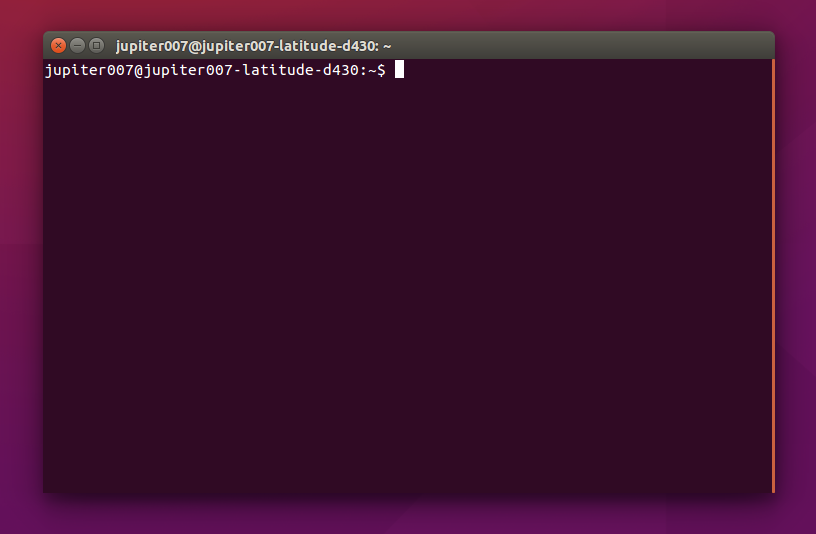
\includegraphics[width=0.8\textwidth]{terminal.png}
\end{center}
\begin{center}
 Console linux pour utiliser Apt-get
\end{center}

\clearpage
\section{Différents gestionnaire}
\subsection{Synaptic}
\paragraph{}
Synaptic est une interface graphique "complète" pour APT. Il permet l'installation de paquets depuis des dépôts APT, de même que leur désinstallation. Les droits d'administration sont nécessaires pour pouvoir utiliser ce programme.
Concrètement il va permettre de chercher et ensuite d'installer automatiquement (presque) tous les programmes que l'on souhaite utiliser. Notez que Synaptic gère des paquets ​provenant de dépôts APT uniquement. Il ne permet ​pas
l'​installation d'un paquet téléchargé manuellement depuis un site Internet ou généré par soi-même. ​

Synaptic est capable de :
\begin{itemize}
\item ajouter ou retirer et activer ou désactiver des dépôts 
\item ajouter, réinstaller ou supprimer des programmes 
\item garder votre système à jour
\end{itemize}
On peut rechercher un paquet dans une liste et on peut voir les paquets disponibles.
\begin{center}

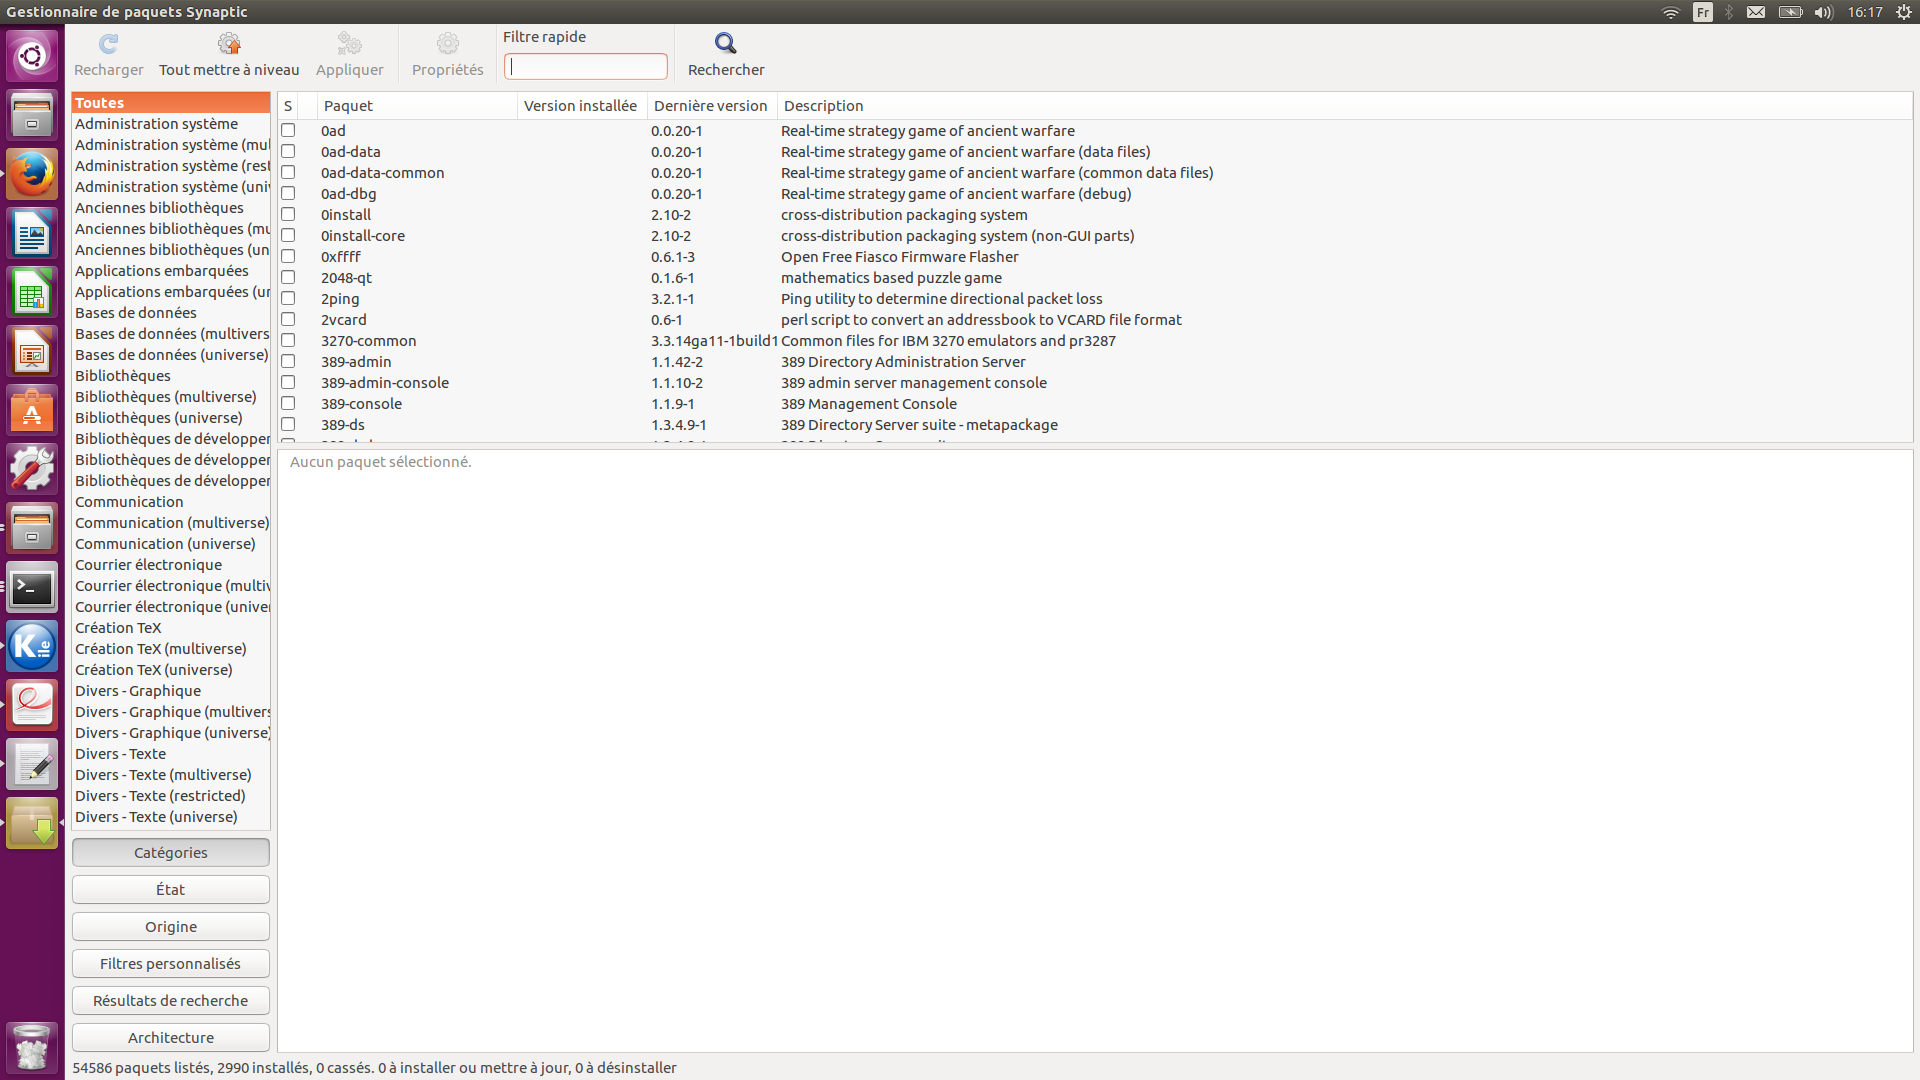
\includegraphics[width=1\textwidth]{synaptic.png}
\end{center}
\begin{center}
 Interface de synaptic
\end{center}


\subsection{Snap}
\paragraph{}
Ubuntu 16.04 est la première version à prendre en charge le nouveau format de paquets logiciels, Snap. Ce format vise à permettre l'installation de nouvelles versions de logiciels dans les systèmes Ubuntu stables, tout en apportant
aux développeurs la facilité de distribution, la fiabilité et la sécurité.
Avec le format Snap, pour recevoir des nouvelles versions de logiciels, les utilisateurs n'auront plus à mettre en jeu la stabilité de leur système Ubuntu par l'ajout de dépôts personnels. Ils pourront récupérer un paquet 
Snappy distribuée par l'éditeur.\\ L'application s'exécute ensuite de manière isolée, ce qui accroît la stabilité et la sécurité du système. Le paquet .snap inclut l'application et peut contenir aussi ses dépendances ; 
en contrepartie d'un paquet plus lourd, ceux-ci peuvent donc faire cohabiter plusieurs versions de mêmes dépendances au sein d'un même système Ubuntu et en facilite la distribution en ligne et hors ligne.
Les paquets Snap ne remplacent pas les paquets Debian : le coeur du système Ubuntu (noyau, environnements graphiques, logiciels de base) continue d'être géré à l'aide des paquets DEB. 
Les paquets Snappy s'ajoutent à l'existant afin de fournir un mode de distribution sûr pour les logiciels tiers ou les versions non validées par le système.

\subsection{Yum}
\paragraph{}
Yum, pour Yellowdog Updater Modified, est un gestionnaire de paquets pour des distributions Linux telles que Fedora, CentOS et Red Hat Enterprise Linux2, créé par Yellow Dog Linux.

Il permet de gérer l'installation et la mise à jour des logiciels installés sur une distribution. C'est une surcouche de RPM gérant les téléchargements et les dépendances, de la même manière que APT de Debian ou Urpmi de Mandriva.
Il existe plusieurs types de paramètres qui peuvent suivre la commande YUM. Certains concernent l'installation (comme install),la suppression (comme remove ), la recherche (search) ou la mise à jour du système (update). Lorsqu'on exécute YUM 
en ligne de commande, cet utilitaire va d'abord interroger un certain nombre de dépôts activés qui sont définis dans le répertoire /etc/yum.repos.d/ ou consulter son cache. En fonction des informations obtenues, il pourra traiter le paramètre qui lui a été ajouté.


\section{Compiler, configurer et installer un logiciel avec les sources}
\paragraph{}

La plupart des programmes sont disponibles à l’aide de la commande apt-get mais certains, trop récent, en développement ou pas assez connus ne le sont pas. 
Il est alors nécessaire de mener des recherche sur le site web du logiciel recherché. \\
On peut alors trouver un fichier en .deb qui permet l’installation d’une programme à la manière d’un .exe sur Windows. Mais ce format est exclusif à Debian et à ses distribution (Ubuntu).
Il existe aussi un format rmp pour Red Hat. Le programme alien permet de de passer d’un format à l’autre.\\
Si le paquetage n’existe pas alors il faut récupérer le code source du programme sur son site. A l’aide du paquet build-essential précédemment installé, nous sommes désormais en mesure d’exécuter ./configure situé dans les fichiers du code source du logiciel que l’on veut installer. 
Cet exécutable permet d’analyser la machine et de vérifier la présence des dépendances du programme.
Si celles-ci ne sont pas toutes présentes, une erreurs apparaît et il faut alors télécharger la dépendance manquante. Une fois que les erreurs sont corrigées il ne reste plus qu’à compiler le programme en tapant make et à l’exécuter en tapant son nom.


\clearpage
\section{Environnement Python}
\subsection{Présentation rapide de l'environnement}
\paragraph{}
Python est un langage de programmation très polyvalent et modulaire, qui est utilisé aussi bien pour écrire des applications comme YouTube, que pour traiter des données scientifiques. Par conséquent, il existe de multiples installations possibles de Python. Par exemple l'une d'entre elle, la suite scientifique Anaconda, rassemble le langage Python et ses modules scientifiques.

\begin{center}
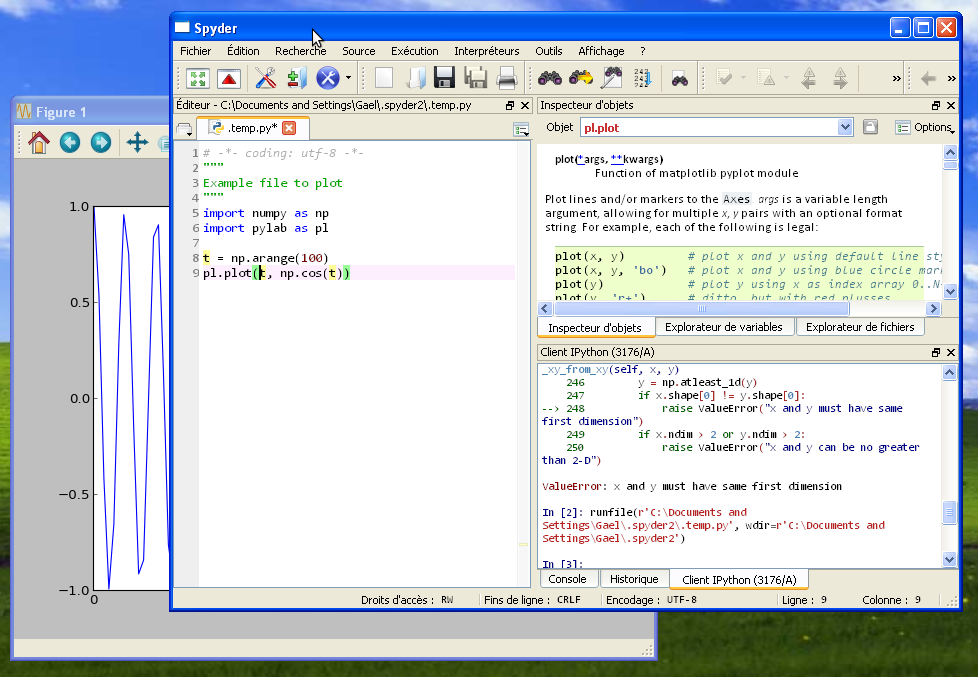
\includegraphics[width=1\textwidth]{EnvPython.png}
 \end{center}
 \begin{center}
 Environnement python
\end{center}


\subsection{L'installation de modules sur Python}
En temps que logiciel libre populaire, Python bénéficie d’une communauté active de contributeurs et d’utilisateurs qui rendent à leur tour leurs logiciels disponibles, sous licence libre, pour les autres développeurs Python.
Cela permet aux utilisateurs de Python de partager et de collaborer efficacement, bénéficiant des solutions que les autres ont déjà crées pour résoudre les problèmes communs (ou même, parfois, rares !), aussi que de partager leurs propres solutions à tous.
Un environnement virtuel est un environnement Python, semi-isolé, qui permet d’installer des paquets pour une application particulière, plutôt que de les installer sur le système entier. Python dispose d'un dépot public, le Python Packaging Index, qui est rendu public par d'autres utilisateurs Python. Ce dépôt public contient des paquets sous licence libre accessibles par tout les utilisateurs de Python.
Voici un exemple de commande pour installer la dernière version d'un module et ses dépendances depuis le Python Package Index:

\begin{verbatim}
 python -m pip install SomePackage==1.0.4 
 // On peut préciser la version minimum ou exacte à installer
\end{verbatim}

Si un module est déjà installé, l'installer à nouveau n'aura aucun effet. La mise à jour de modules doit être demandée par la ligne de commande suivante:

\begin{verbatim}
 python -m pip install --upgrade SomePackage
\end{verbatim}
L'installation de paquets peut se faire seulement pour l'utilisateur actuel: l'installation ne se fera pas pour tous les utilisateurs du système. Pour cela, il faut rajouter l'option --user à la commande python -m pip install.

\subsection{Les problèmes d'installation typiques}
- Sur les systèmes Linux, une installation de Python sera généralement inclue dans le cadre de la distribution. Installer dans cette installation de Python nécessite un accès root sur le système, et peut interférer avec le fonctionnement du gestionnaire de paquets du système et d’autres composants du système si un composant est mis à jour de façon inattendue en utilisant pip.

Sur de tels systèmes, il est souvent préférable d’utiliser un environnement virtuel ou une installation par l’utilisateur lors de l’installation des paquets avec pip.

- Problème lors de l'installation d'extensions binaires:
Python a généralement beaucoup misé sur une distribution basée sur les sources, avec laquelle les utilisateurs finaux devaient compiler, lors de l’installation, les modules d’extension à partir des sources.

Avec l’introduction du format binaire wheel, et la possibilité de publier des wheels, pour, au moins Windows et Mac OS X, via le Python Package Index, ce problème devrait diminuer au fil du temps, car les utilisateurs sont plus régulièrement en mesure d’installer des extensions pré-compilées plutôt que de devoir les compiler eux-mêmes.

\clearpage
\section{Références}


\url{https://framasoft.org/article2460.html}\\
\url{https://doc.ubuntu-fr.org/synaptic}\\
\url{https://doc.ubuntu-fr.org/apt-get}\\
\url{https://doc.ubuntu-fr.org/depots}\\
\url{https://doc.ubuntu-fr.org/gestionnaire_de_paquets}\\
\url{http://doc.fedora-fr.org/wiki/YUM_:_Configuration_du_gestionnaire_de_paquets}\\
\url{https://openclassrooms.com/courses/reprenez-le-controle-a-l-aide-de-linux/compiler-un-programme-depuis-les-sources}\\
\url{http://python-prepa.github.io/intro.html}\\
\url{https://www.afpy.org/doc/python/2.7/installing/index.html}\\

\end{document}
